\section{Introduction}

\begin{frame}
\frametitle{Surgical Robotics Procedure}
\begin{columns}
\column{0.32\textwidth}
\begin{center}
\begin{figure}[htbp]
\centering
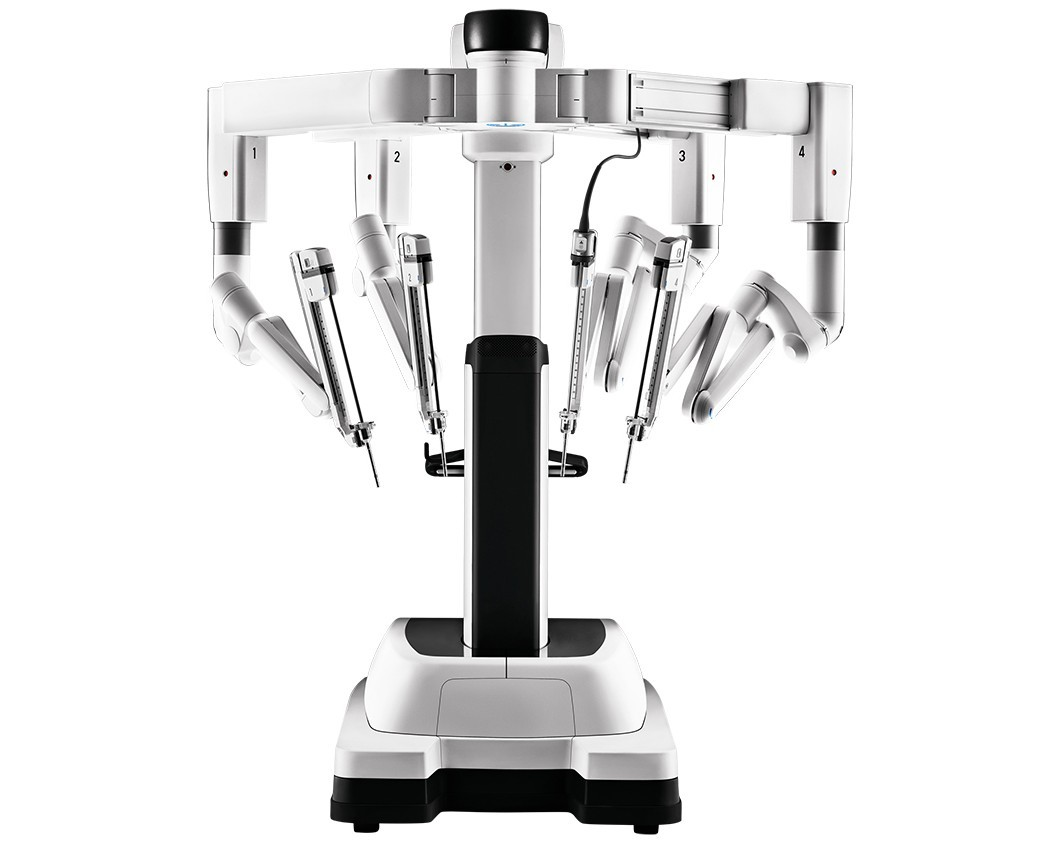
\includegraphics[width=\textwidth]{../images/intuitive-da-vinci-xi-patient-cart-front-view-1060867-lo-res.jpg}\\
\caption{DaVinci Xi, \textsuperscript \textcopyright 2020 Intuitive Surgical, Inc.}
\end{figure}
\end{center}
\column{0.32\textwidth}
\begin{center}
\begin{figure}[htbp]
\centering
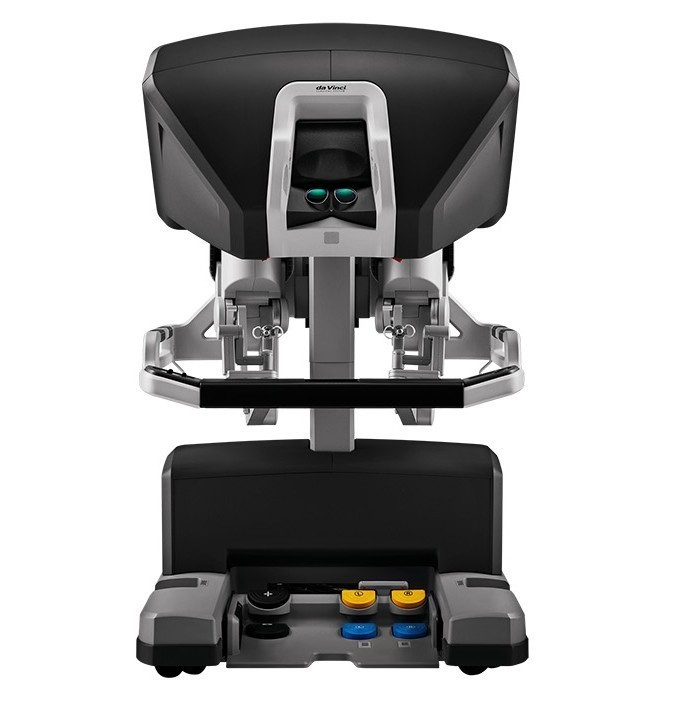
\includegraphics[width=\textwidth]{../images/intuitive-davinci-console-front-lowres.jpg}\\
\end{figure}
\end{center}
\column{0.32\textwidth}
\begin{enumerate}
\item patient preparation
\item small incisions at the anatomical region of interest
\item trocars mounting
\item robot positioning, mounting \& calibration of surgical tools
\item remote operation from special console
\end{enumerate}
\end{columns}
\end{frame}

\begin{frame}
\frametitle{Advantages of Surgical robotics}
\begin{columns}[t]
\column{0.5\textwidth}
for the patient, \textbf{Minimally Invasive}:
\begin{itemize}
\item Smaller incisions
\item Less blood loss
\item Reduced risk of inpatient infection
\item Less pain
\item Faster patient recovery
\end{itemize}

\column{0.5\textwidth}
for the surgeon:
\begin{itemize}
\item Increased \textbf{precision} and reduced human errors: Smooth and precise movements, Detection and correction of errors caused by hand tremble
\item \textbf{No fulcrum effect}
\item Haptic feedback
\item Teleoperation \& ergonomics
\end{itemize}
\end{columns}
\end{frame}

\begin{frame}
\frametitle{Thesis goals}
Study all the stages involved in the perception, control and manipulation of robotic laparoscopic tools with emphasis given to the \textbf{pivot trajectories and the RCM constrained motion planning}
\begin{itemize}
\item laparoscopic tool detection, calculation of relative position and orientation of the center of mass
\item calculate the contact points on the tool
\item calculate the path from the tools’ table to the surgical table
\item calculate the pivot trajectories that needs to be executed when the tool is inserted in the trocar
\end{itemize}
\end{frame}